\documentclass[conference]{IEEEtran}
\IEEEoverridecommandlockouts
% The preceding line is only needed to identify funding in the first footnote. If that is unneeded, please comment it out.

\usepackage{booktabs}
\usepackage{amsmath,amssymb,amsfonts, mathabx}
% \usepackage[backend=biber,style=alphabetic,sorting=ynt]{biblatex}
% \addbibresource{sample.bib} %Import the bibliography file
\usepackage{enumitem}
\usepackage{algorithmic}
\usepackage{physics}
\usepackage{graphicx}
\usepackage{textcomp}
\usepackage[colorlinks=true, allcolors=black]{hyperref}
\usepackage{xcolor}
\usepackage{multirow}
\def\BibTeX{{\rm B\kern-.05em{\sc i\kern-.025em b}\kern-.08em
    T\kern-.1667em\lower.7ex\hbox{E}\kern-.125emX}}
\begin{document}
\title{Model Predictive Control for Trajectory Tracking Mini-quadcopters\\}
\author{\IEEEauthorblockN{Akash John Subash}
\IEEEauthorblockA{\textit{M.Sc. Embedded Systems Engineering}}
}

\maketitle

\begin{abstract}
This project report formulates a setpoint tracking controller computed in real-time using Model Predictive Control (MPC). It subsequently proposes a trajectory tracking scheme achieved by a path parametric model reformulation using the Frenet-Serret transforms while retaining convex geometric collision constraints in the Cartesian coordinate frame.

\end{abstract}

\section{Introduction}\label{Introduction}
The Crazyflie 2.1 quadcopter is a versatile open-source flying development platform with expansion decks that make it a good candidate for university projects. The optimal controls computed offboard using MPC are fed to the crazyFlie, with the intention to overtake a second quadcopter (henceforth referred to as obstacle).

This Section continues by describing the related work Section \hyperref[Section2]{II} describes the model and the dynamics of the crazyFlie 2.1 quadcopter using Ordinary Differential Equations (ODE). Section \hyperref[Section3]{III} details the optimal control problem, its non-linear program and section \hyperref[Section4]{IV}, \hyperref[Section5]{V} illustrate the control topologies in open and closed-loop. Section \hyperref[Section6]{VI} presents the results of simulation and flight tests. Section \hyperref[Section7]{VII} presents the results of simulation and flight tests and Section Section \hyperref[7]{VII} outlines the ongoing reformulation for trajectory tracking and its subsequent timeline. 
\section{System Modelling}\label{Section2}
\begin{figure}[htbp]
	\centerline{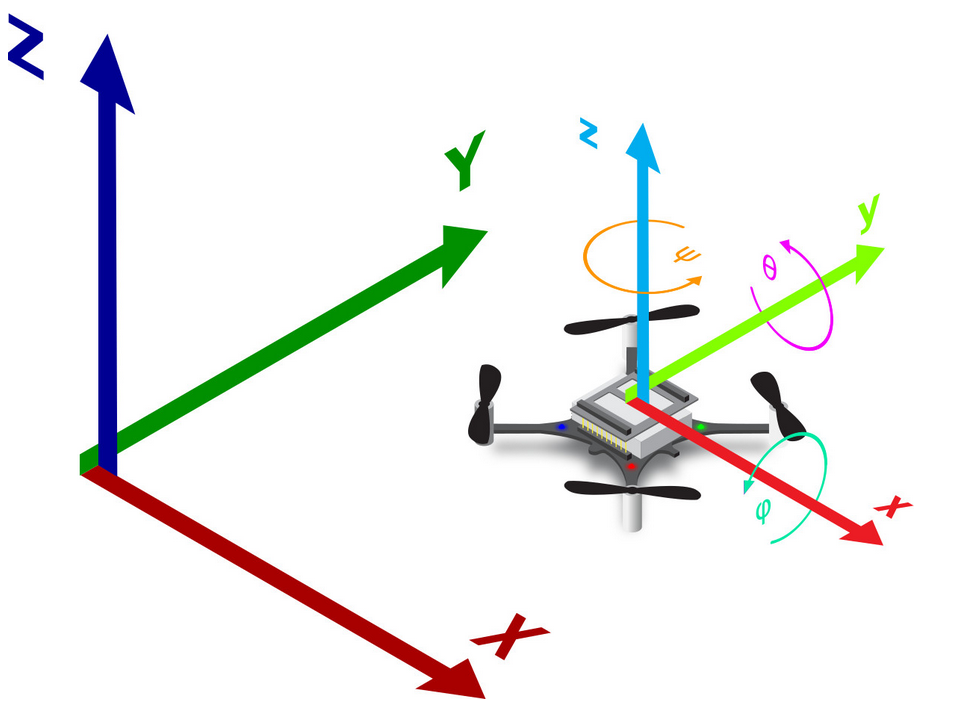
\includegraphics[scale = 0.4]{figures/ordinate.png} }
	\caption{Reference coordinate system [1]}
	\label{Fig1}
\end{figure}
As depicted in \hyperref[Fig1]{Fig. 1}, a body frame located at the center of mass of the quadcopter aligned with the East-North-Up inertial frame is used here, with $\varphi$, $\theta$, $\psi$ representing roll, pitch and yaw in the Euler notation respectively.

\subsection{Dynamic Model}
The state ${\zeta\,\in\,\mathbb{R}\,\mathrm{^{13}}}$ of the drone described by position ${p = (x, y, z)\mathrm{^{T}}}$ in the inertial frame, attitude in quaternion $q = (q_{0}, q_{1}, q_{2}$, $q_{3})\mathrm{^{T}}$, transalational velocities $v = (v_x, v_y, v_z)\mathrm{^{T}}$, and angular velocities $\omega = (\omega_{\phi}, \omega_{\theta}, \omega_{\psi})\mathrm{^{T}}$ in the body frame. Its non-linear dynamics adapted from \cite{carlos_efficient_2020} are given by the ODEs 

\begin{align}
\dot{\zeta} &= \begin{bmatrix}
	\dot{p} \\
	\dot{q}\\
	\dot{v}\\
	\dot{\omega}
\end{bmatrix} =
\begin{bmatrix}
    Sv \\
    \dfrac{1}{2}q\times \omega\\
    \dfrac{1}{m}F - S\mathrm{^{T}}g1_z - \omega \times v\\ 
    J\mathrm{^{-1}}(M - \omega \times J \omega)
\end{bmatrix}.
\end{align}

The model parameters described in \hyperref[table1]{Table I} are used in conjunction with the quaternion rotation matrix ${S\,\in\,\mathbb{R}\,\mathrm{^{3\times3}}}$, external force matrix ${F\,\in\,\mathbb{R}\,\mathrm{^{3\times1}}}$, external momentum matrix ${M\,\in\,\mathbb{R}\,\mathrm{^{3\times1}}}$, and moment of inertia matrix ${J\,\in\,\mathbb{R}\,\mathrm{^{3\times3}}}$ as

\begin{align}
	S &= 2 \cdot
	\begin{bmatrix}
		q_{0}^{2} + q_{1}^{2} - \dfrac{1}{2} & 
		q_1 q_2 - q_0 q_3 & 
		q_0 q_2 + q_2 q_3 \\
		q_0 q_3 + q_1 q_2 &
		q_{0}^{2} + q_{2}^{2} - \dfrac{1}{2} & 
		q_2 q_3 - q_0 q_1 \\
		q_1 q_3 - q_0 q_2 & 
		q_0 q_1 + q_2 q_3 & 
		q_{0}^{2} + q_{3}^{2} - \dfrac{1}{2}\\
	\end{bmatrix}
\end{align}

\begin{align}
	F &=
	\begin{bmatrix}
		0 \\
		0 \\
		C_t(\Omega_1\mathrm{^{2}} + \Omega_2\mathrm{^{2}} + \Omega_3\mathrm{^{2}} + \Omega_4\mathrm{^{2}})\\ 
	\end{bmatrix}
\end{align}

\begin{align}
	J &=   
	\begin{bmatrix}
		I_{x} & 0 & 0\\
		0 & I_{y} & 0\\
		0 & 0 & I_{z}\\ 
	\end{bmatrix}
\end{align}

\begin{align}
	M &=
	\begin{bmatrix}
		\frac{1}{\sqrt{2}}\,dC_t(-\Omega_1\mathrm{^{2}} - \Omega_2\mathrm{^{2}} + \Omega_3\mathrm{^{2}} + \Omega_4\mathrm{^{2}})\\
		\frac{1}{\sqrt{2}}\,dC_t(-\Omega_1\mathrm{^{2}} + \Omega_2\mathrm{^{2}} + \Omega_3\mathrm{^{2}} - \Omega_4\mathrm{^{2}})\\
		C_d(-\Omega_1\mathrm{^{2}} + \Omega_2\mathrm{^{2}} - \Omega_3\mathrm{^{2}} + \Omega_4\mathrm{^{2}})
	\end{bmatrix}.
\end{align}
Given the possibility to individually change the angular velocities of the propellers, the control vector is defined as: \\
$u$ := ($\Omega_{1}$, $\Omega_{2}$, $\Omega_{3}$, $\Omega_{4}$)$\mathrm{^{T}}$ $\in$ $\mathbb{R}\mathrm{^{4}}$

\begin{table}[htbp]
	\small
	\begin{center}
		\begin{tabular}{lccccl}\toprule
			\textbf{Description} &  \textbf{Symbol}\\
			\midrule
            $\mathrm{Mass\,of\,the\,drone} \,m$ & $\mathrm{31 \cdot 10^{-3}\,\mathrm{kg}}$  \\
			$\mathrm{Drone\,arm\,length} \,d$ & $46 \cdot \mathrm{10^{-3}}\,\mathrm{m}$ \\
			$\mathrm{Inertial\,moment} \,I_{x}$ & $1.395 \cdot\,\mathrm{10^{-5}} \mathrm{kg\,m^2}$ \\
            $\mathrm{Inertial\,moment} \,I_{y}$ & $1.395 \cdot\,\mathrm{10^{-5}} \mathrm{kg\,m^2}$ \\
            $\mathrm{Inertial\,moment} \,I_{z}$ & $2.173 \cdot\,\mathrm{10^{-5}} \mathrm{kg\,m^2}$ \\
            $\mathrm{Coefficient\,of\,drag} \,C_d$ & $\mathrm{7.93 \cdot 10^{-12}}\,\mathrm{N\,RPM^{-2}}$ \\
			$\mathrm{Coefficient\,of\,thrust} \,C_t$ & $\mathrm{3.25 \cdot 10^{-10}}\,\mathrm{N\,RPM^{-2}}$ \\
			$\mathrm{Gravitational\,acceleration} \,g$ & $\mathrm{9.81 \cdot\,m\,s^{-2}}$ \\
			\bottomrule
		\end{tabular}
	\end{center}
	\caption{Parameters of the model}
	\label{table1}
\end{table}

\begin{figure*}[htbp]
	\centerline{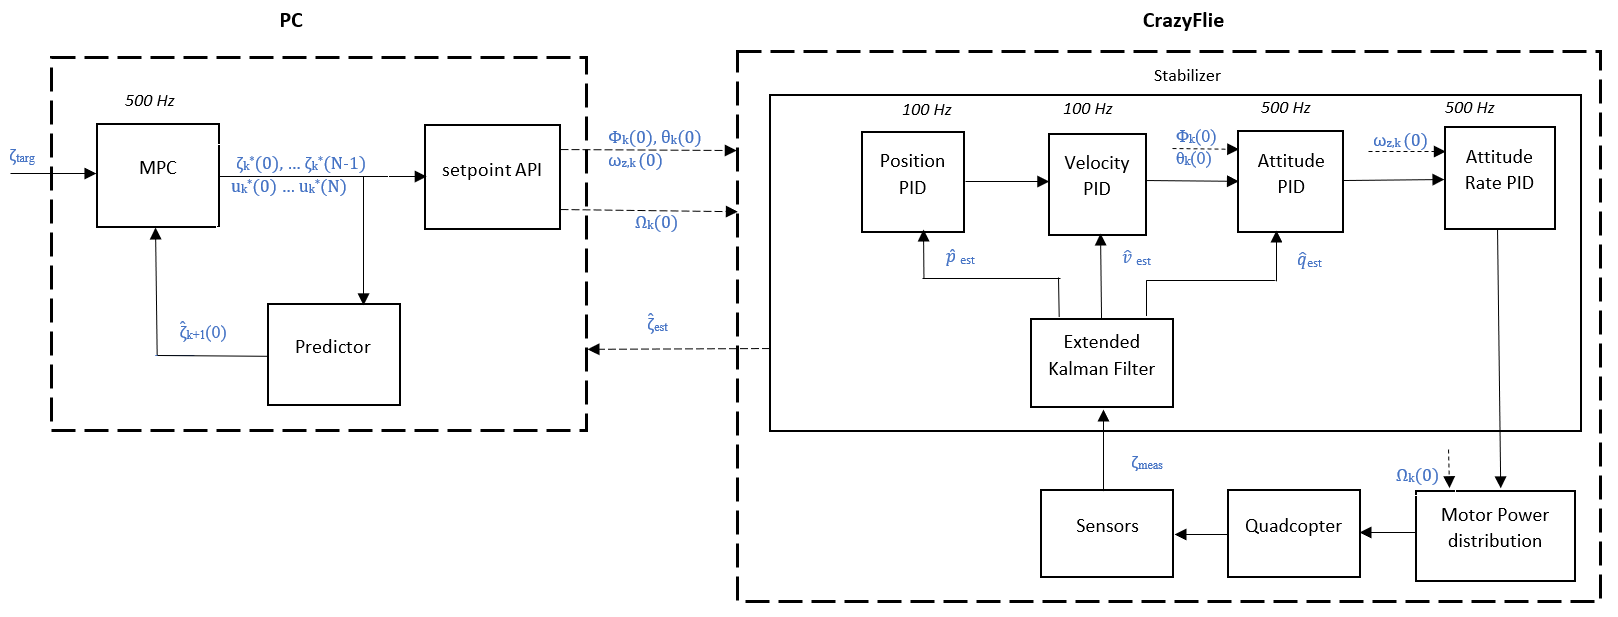
\includegraphics[scale = 0.6]{figures/Screenshot_OL.png} }
	\caption{Open loop control architecture }
	\label{Fig2}
\end{figure*}

\subsection{Delay Compensation}


The round trip delay which is computed as the sum of radio communication latency between the off-board processor and the quadcopter, and solving the NLP ( $\tau_{rr}$ = $\tau_{t}$ + $\tau_{r}$ + $\tau_{c}$) needs to be compensated to retain claims of optimality. The inherent challenge of measuring one-way latency is accounted for and handled as in \cite{carlos_efficient_2020} by introducing a delay compensation block marked as predictor in Figure 2.

\section{Problem Formulation}\label{Section3}

In this section, the discretized Optimal Control Problem (OCP) and its constrained Non-Linear Program (NLP) are defined using direct multiple shooting \cite{bock_multiple_1984} to discretize the underlying continuous-time OCP.

\subsection{Optimal Control Problem}

The initial state is defined as the quadcopter hovering at a height $z$ = 0.5 m, and the goal is to reach a specified target state avoiding another quadcopter along the way, at position  $p_\mathrm{b}$ = ($x_\mathrm{b}$, $y_\mathrm{b}$, $z_\mathrm{b}$)$\mathrm{^{T}}$

The discretized cost function is defined as :
\begin{align}
	& L\left(\zeta_k, U_k\right) = \lVert \zeta_k - \zeta_{\mathrm{trg}} \rVert^2_Q + \lVert u_k - u_{\mathrm{hov}} \rVert^2_R
\end{align}

The OCP is then formulated as :
\begin{align}
	&\min_{u_0,\zeta_0,..,u_{N-1},\zeta_N} \quad \sum_{k = 0}^{N-1} L(\zeta_k, u_k) \\
	\text{s.t} \quad
	& \zeta_0 - \bar{\zeta_0} \hspace{0.42in} = 0\\
    & \zeta_k - F(\zeta_k, u_k) = 0, \hspace{0.1in}\quad\qquad k = 0,..,N-1 \\
    & 3\,\mathrm{d} \hspace{0.1in} \le \lVert p_k - p_{\mathrm{b}} \rVert, \qquad \qquad  k = 0,..,N-1 \\
	& \zeta_{\mathrm{min}} \le \hspace{0.22in} \zeta_k \hspace{0.25in} \le \zeta_{\mathrm{max}}, \quad k = 0,..,N-1 \\
    & 0 \hspace{0.2in} \le \hspace{0.23in} u_k \hspace{0.22in} \le U_{\mathrm{max}} \quad k = 0,..,N-1
\end{align}

\begin{flushleft}
$\bar{\zeta_0}$ \hspace{0.18in}= $(0, 0, 0.5, 1, 0, 0, 0, 0, 0, 0, 0, 0, 0)^T$\\
$\zeta_{\mathrm{trg}}$ \hspace{0.08in}= $( 1, 1, 1, 1, 0, 0, 0, 0, 0, 0, 0, 0, 0)^T$\\
$\zeta_{\mathrm{max}}$ \hspace{0.03in}= $(1.5,1.5,1.5,\infty,\infty,\infty,\infty,0.25,0.25,0.25,\frac{\pi}{4},\frac{\pi}{4},\frac{\pi}{4})^T$\\
$\zeta_{\mathrm{min}}$ \hspace{0.05in}= -$\zeta_{\mathrm{max}}$\\
$U_{\mathrm{max}}$ = $(22000, 22000, 22000, 22000)^T$\\
$p_\mathrm{b}$ \hspace{0.18in}= $(0.5, 0.5, 0.5)^T$\\
\end{flushleft}

 $\zeta := (\zeta_0, .., \zeta_N)^T$, and $u := (u_0, .., u_{N-1})^T$ denote the state and control trajectories of the dynamics descretized by the RK4 integrator $F :$ $\mathbb{R}^{n_{\zeta}} \cdot \mathbb{R}^{n_{u}} \rightarrow \mathbb{R}^{n_{\zeta}}$. The horizon length and the estimated state of the system at the current time instant $k$ are denoted by $N$, and $\zeta_k$ respectively.

 $Q$ $\in$ $\mathbb{R}^{n_{\zeta} \cdot n_{\zeta}}$ and $R$ $\in$ $\mathbb{R}^{n_{u} \cdot n_{u}}$ are positive definite weighting matrices, tuned experimentally for the specific flight path.
\begin{flushleft}
\begin{small}
$Q$ = diag\begin{footnotesize}$(120, 100, 100, 10^{-3}, 10^{-3},10^{-3},1, 1, 1, 1, 10^{-5}, 10^{-5}, 10^{-5})$\\
\end{footnotesize}
$R$ = diag\begin{footnotesize}$(8 \cdot 10^{-1}, 8\cdot 10^{-1}, 8\cdot 10^{-1}, 8\cdot 10^{-1})$\\
\end{footnotesize}
\end{small}
\end{flushleft}

% \section{Open-loop Control }\label{Section4}
% The open-loop control of the drone without the obstacle to be avoided was implemented with a horizon of $N = 10$ in Python using the CasADi \cite{andersson_casadi_2019} framework with IPOPT \cite{wachter_implementation_2006} as the interior point NLP solver. Using the next state predicted by the RK4 integrator from the current state and controls, the MPC computes the optimal solution iteratively. The optimal open-loop controls for each time could only be fed with minimal delay to the quadcopter, by solving the problem offline.

% However, the large error propagation causing the quadcopter to quickly veer off the estimated trajectory, warrants the closed loop problem, and argues against placing the obstacle in the quadcopter's flight path in open-loop.
% The appropriate set-point command API provided by the open-source crazyFlie libraries allowed to communicate the controls as a set of roll, pitch, yaw rate, and thrust.

\section{Closed-loop Control }\label{Section5}
Using IPOPT \cite{wachter_implementation_2006} as the interior point NLP solver, the estimated state from the Extended Kalman filter onboard the Crazyflie sampled at 50 Hz, was fed back with delay compensation for closed-loop control. The sampling rate was determined by the lower bound on the achievable computation time of the solver. Using MPC to control the system, an instance of (2) is solved iteratively at each sampling time point, with the current value of the state estimate $\zeta_k$.

The closed loop architecture differs from Figure 2, only in the feedback path, where the predictor computes $\hat{\zeta}_{k+1}$ from $\hat{\zeta}_{\mathrm{est}}$ instead of $\zeta^*_{k}$.
In closed-loop, adding the obstacle to be avoided necessitated increasing the horizon to $N$ = 20 for a smooth control, and state trajectory which led to a large increase in computation time ($\tau_c$).

\section{Closed-loop Control Results}\label{Section6}

The most important factor to consider while moving from simulations to hardware flights were delays. The choice of
$\tau_s$ was made to ensure the quadcopter's state, control trajectory evolution were plausible, while trying to maintain a minimal $\tau_c$. A value of $\tau_s$ = 20 ms was found to provide a good trade-off between the two.
The round trip delay $\tau_{trr}$ was found to be dominated by $\tau_{c}$ which is dependant on the choice of the solver framework, and the integration step ($\tau_s$) of the non-linear system dynamics, and most importantly, the OCP formulation.

% \begin{figure}[htbp]
% 	\centerline{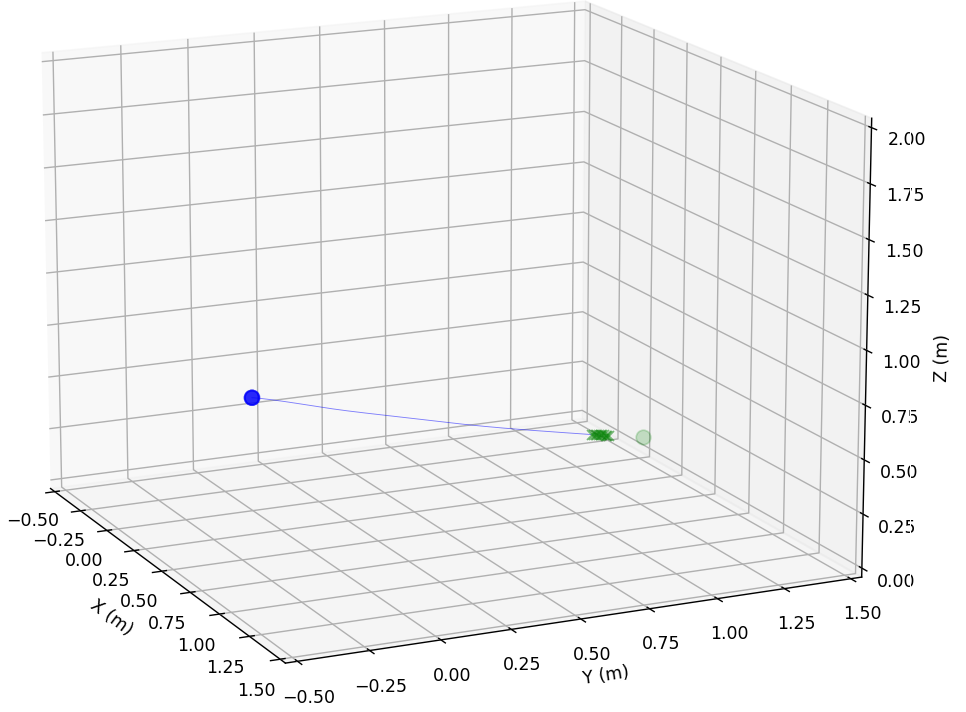
\includegraphics[scale = 0.4]{figures/Screenshot_OL_ST.png} }
% 	\caption{Open loop trajectory without obstacle for $N$ = 10, $\tau_s$ = 20ms}
% 	\label{Fig3}
% \end{figure}

\begin{figure}[t!]
    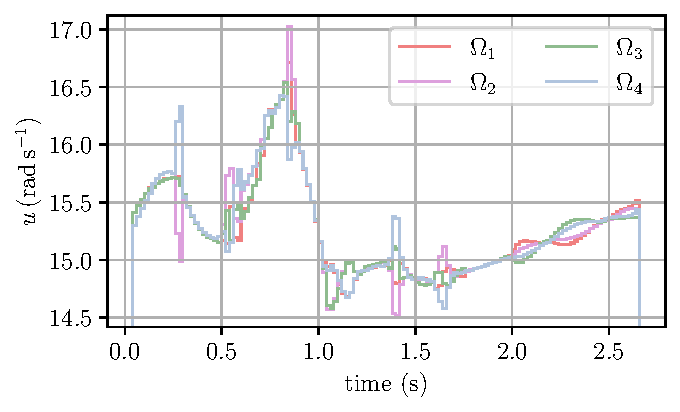
\includegraphics[width=0.48\textwidth]{figures/u.pdf}
    \caption{Open loop control $(u)$ with obstacle for $N$ = 20, $\tau_s$ = 20ms, $\tau_c$ = 40ms}  \label{fig_comp_zeta_u_AGV}
\end{figure}

\begin{figure}[htbp]
	\centerline{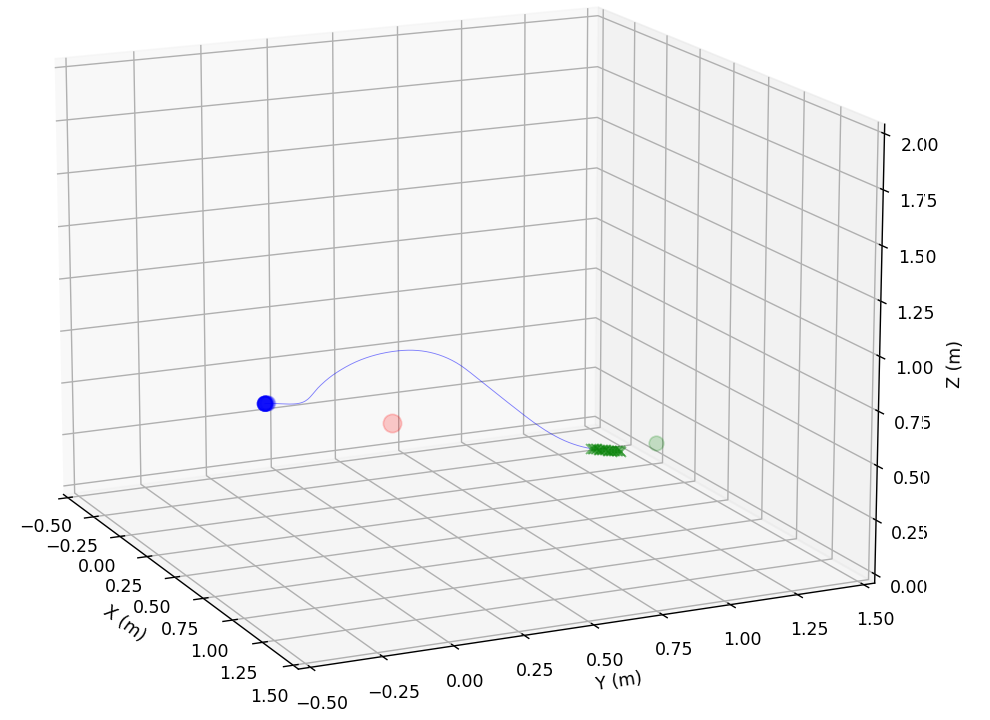
\includegraphics[scale = 0.4]{figures/Screenshot_OLwO_ST.png} }
	\caption{Open loop substate vector $p$ with obstacle for $N$ = 20, $\tau_s$ = 20ms}
	\label{Fig4}
\end{figure}

In the open, and closed loop flights without the obstacle, $\tau_{trr}$ was sufficiently small to observe stable flights. In closed-loop, with the obstacle and $N$ = 10, the quadcopter's attempt at aggressively avoiding the obstacle caused large jumps in the state estimate, impacting solution convergence. With $N$ = 20 shooting nodes smoother control trajectories were observed at the expense of a large $\tau_{c}$, compromising the controller's real-time feasibility.

% \begin{figure*}[t!]
% 	\centerline{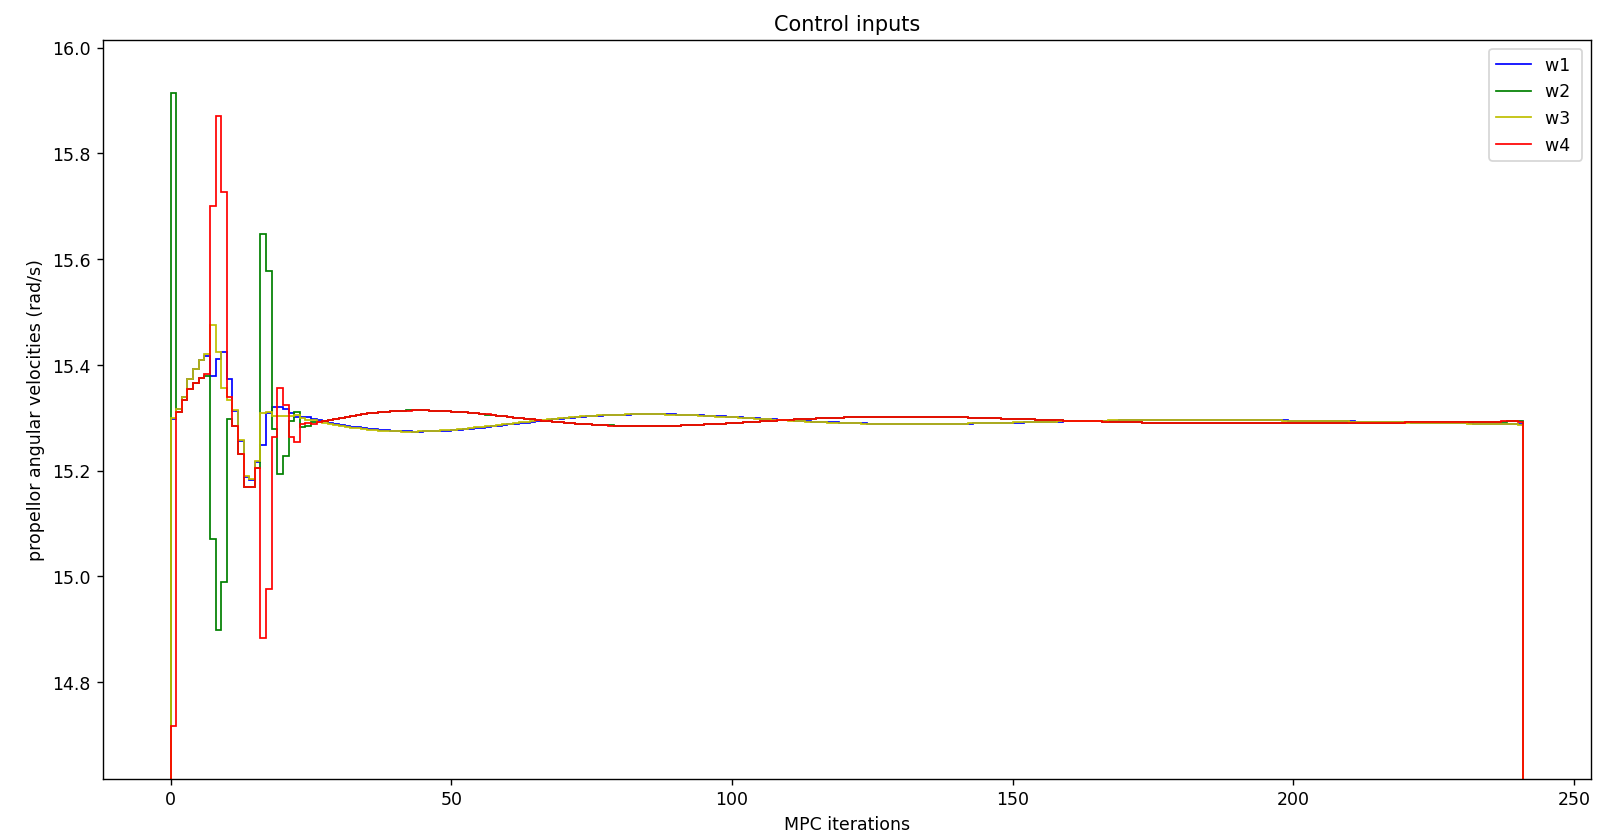
\includegraphics[scale = 0.45]{figures/Screenshot_OL_U.png} }
% 	\caption{Open loop controls without obstacle for $N$ = 10, $\tau_s$ = 20ms, $\tau_c$ = 40ms}
% 	\label{Fig5}
% \end{figure*}

The average closed-loop iteration times were $\tau_{c}$ = 40 ms, and $\tau_{c}$ = 100 ms without and with active collision constraints on an Intel i7-8750H processor @2.2Ghz running Windows.
\section{Proposal}\label{Section7}
\par For a more intuitive representation of progress we propose the spatial reformulation of the dynamics in the Frenet Coordinate Frame as in \cite{arrizabalaga_towards_2022} while retaining convex constraint guarantees using the lifted and direct elimination controllers as in \cite{reiter_frenet-cartesian_2023}. The convergence properties of the coordinate transformed encoding of the environment is proven to be superior for progress maximization problems in \cite{werling_invariant_2010}.
To achieve a real-time feasible scheme we aim to use hardware-tailored linear algebra libraries \cite{frison_blasfeo_2018} in acados \cite{verschueren_acados_2020} with the real-time iteration \cite{gros_linear_2020} (RTI) and partial condensing to exploit the structured QP subproblem \cite{frison_hpipm_2020}
Subsequently, the constraint tightening shows promise for improved convergence of the demanding geometric collision constraints.
\bibliographystyle{ieeetr}
\bibliography{./bibliography/sample.bib}
\end{document}

% git commit --amend
% git rebase -i revision